\documentclass{standalone}
\usepackage[none]{hyphenat}
\usepackage{tikz}
\usetikzlibrary{positioning}
\usetikzlibrary{calc}
\usetikzlibrary{fit}
\usetikzlibrary{shapes}
\usetikzlibrary{arrows}
\usetikzlibrary{intersections}
\usetikzlibrary{shapes.geometric}
\usetikzlibrary{decorations.pathreplacing}

\tikzset{>=latex}
\tikzset{transaction/.style={font=\small{#1}}}
\tikzset{square/.style={regular polygon,regular polygon sides=4}}
\tikzset{key/.style={rectangle, draw, minimum height=10pt, text width=2cm, align=center}}
\tikzset{hash/.style={rectangle, draw, minimum height=10pt, text width=1cm, align=center}}
\tikzset{signature/.style={rectangle, draw, minimum height=10pt, text width=2cm, align=center}}

\tikzset{stage/.style={square, draw, minimum height=14pt, text width=2.0cm, align=center}}
\tikzset{title/.style={font=\bfseries}}

\begin{document}
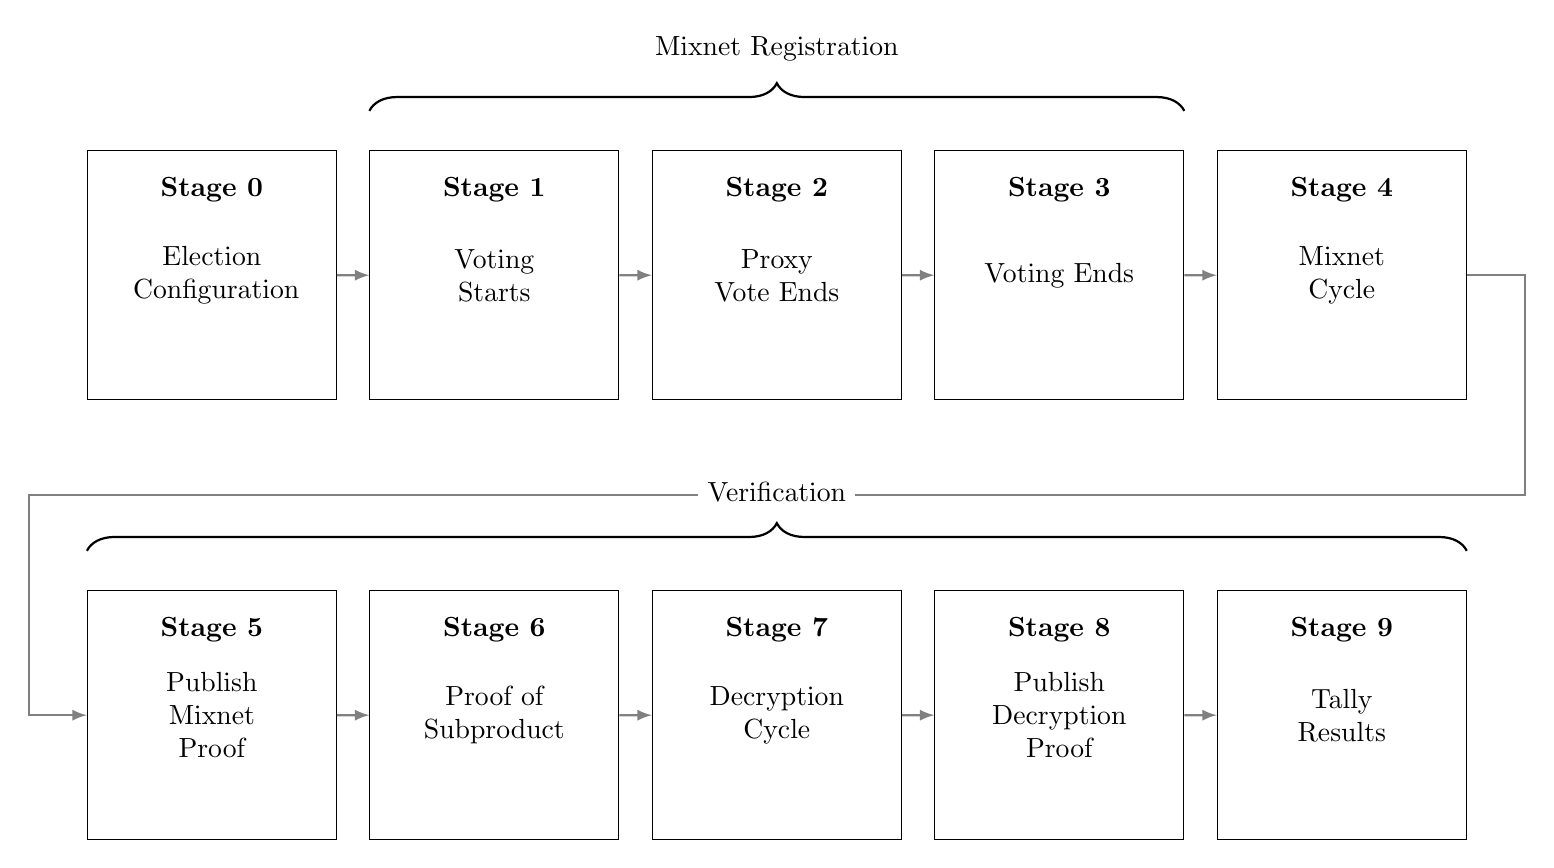
\begin{tikzpicture}[remember picture]

    % Nodes
    \node [stage] (stage0) at (10,10) {Election Configuration};
    \node [stage] (stage1) at ($(stage0.east) + (2, 0)$) {Voting Starts};
    \node [stage] (stage2) at ($(stage1.east) + (2, 0)$) {Proxy Vote Ends};
    \node [stage] (stage3) at ($(stage2.east) + (2, 0)$) {Voting Ends};
    \node [stage] (stage4) at ($(stage3.east) + (2, 0)$) {Mixnet Cycle};
    \node [stage] (stage5) at ($(stage0.south) + (0, -4)$) {Publish Mixnet Proof};
    \node [stage] (stage6) at ($(stage5.east) + (2, 0)$) {Proof of Subproduct};
    \node [stage] (stage7) at ($(stage6.east) + (2, 0)$) {Decryption Cycle};
    \node [stage] (stage8) at ($(stage7.east) + (2, 0)$) {Publish Decryption Proof};
    \node [stage] (stage9) at ($(stage8.east) + (2, 0)$) {Tally Results};

    % Stage titles
    \node [title] () at ($(stage0.north) + (0, -0.5)$) {Stage 0};
    \node [title] () at ($(stage1.north) + (0, -0.5)$) {Stage 1};
    \node [title] () at ($(stage2.north) + (0, -0.5)$) {Stage 2};
    \node [title] () at ($(stage3.north) + (0, -0.5)$) {Stage 3};
    \node [title] () at ($(stage4.north) + (0, -0.5)$) {Stage 4};
    \node [title] () at ($(stage5.north) + (0, -0.5)$) {Stage 5};
    \node [title] () at ($(stage6.north) + (0, -0.5)$) {Stage 6};
    \node [title] () at ($(stage7.north) + (0, -0.5)$) {Stage 7};
    \node [title] () at ($(stage8.north) + (0, -0.5)$) {Stage 8};
    \node [title] () at ($(stage9.north) + (0, -0.5)$) {Stage 9};

    % Arrows between nodes
    \draw [->,gray,thick] (stage0) -- (stage1);
    \draw [->,gray,thick] (stage1) -- (stage2);
    \draw [->,gray,thick] (stage2) -- (stage3);
    \draw [->,gray,thick] (stage3) -- (stage4);
    \draw [->,gray,thick] (stage5) -- (stage6);
    \draw [->,gray,thick] (stage6) -- (stage7);
    \draw [->,gray,thick] (stage7) -- (stage8);
    \draw [->,gray,thick] (stage8) -- (stage9);
    % Middle arrow
    % \draw [->,gray,thick] (stage4) |- (verification) -| (stage5);
    \coordinate (middle) at ($(stage2)!0.5!(stage7) + (0,0.0)$);
    \coordinate (middle-east) at ($(middle) + (9.5,0)$);
    \coordinate (middle-west) at ($(middle) - (9.5,0)$);
    % \draw [->,thick,gray] (stage4) |- (middle-west) |- (stage5.west);
    \draw [->,thick,gray] (stage4.east) -| (middle-east) -- (middle-west) |- (stage5.west);

    % 1st curly brace
    \draw [decorate,decoration={brace,amplitude=10pt},thick]
        ($(stage1.north west) + (0, 0.5)$) --
        ($(stage3.north east) + (0, 0.5)$)
        node [black,midway,above,yshift=0.5cm] {Mixnet Registration};

    % 2nd curly brace
    \draw [decorate,decoration={brace,amplitude=10pt},thick]
        ($(stage5.north west) + (0, 0.5)$) --
        ($(stage9.north east) + (0, 0.5)$)
        node [black,midway,above,yshift=0.5cm,fill=white] (verification) {Verification};


    % Bottom arrow
%    \draw[>=triangle 90, thick, ->] ($(stage0.south west) + (0, -0.5)$) --
%                                    ($(stage9.south east) + (0, -0.5)$)
%                                    node [below] {}; % Node so the arrow head doesn't get cropped.

\end{tikzpicture}
\end{document}
